%###############################################################################
%# N1 - Manual - Stacks                                                        #
%###############################################################################
%#    Copyright 2018 Dirk Heisswolf                                            #
%#    This file is part of the N1 project.                                     #
%#                                                                             #
%#    N1 is free software: you can redistribute it and/or modify               #
%#    it under the terms of the GNU General Public License as published by     #
%#    the Free Software Foundation, either version 3 of the License, or        #
%#    (at your option) any later version.                                      #
%#                                                                             #
%#    N1 is distributed in the hope that it will be useful,                    #
%#    but WITHOUT ANY WARRANTY; without even the implied warranty of           #
%#    MERCHANTABILITY or FITNESS FOR A PARTICULAR PURPOSE.  See the            #
%#    GNU General Public License for more details.                             #
%#                                                                             #
%#    You should have received a copy of the GNU General Public License        #
%#    along with N1.  If not, see <http:%www.gnu.org/licenses/>.               #
%###############################################################################
%# Version History:                                                            #
%#   Novemmber 27, 2018                                                        #
%#      - Initial release                                                      #
%###############################################################################

\section{Stacks}
\label{stacks}

The N1 operates with two stacks: the \gls{ps} to perform data transactions and the
\gls{rs} to manage the program flow. As illustrated in \figref{stacks:fig}, each of
these stacks consists of three segments: the \gls{us}, the \gls{is}, and the \gls{ls}.

\begin{figure}[!h]
  \begin{center}
  \makebox[\textwidth][c]{
    \scalebox{1} {
      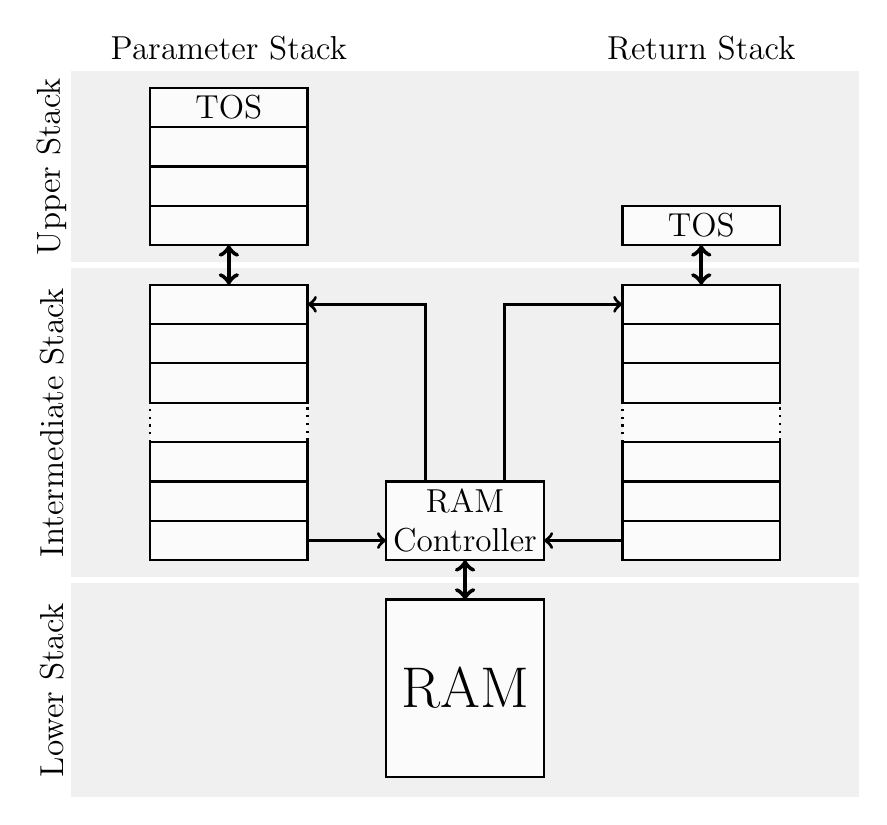
\begin{tikzpicture}

        %Lower stack
        \draw [gray!12, fill=gray!12](0.5,0)   rectangle (10.5,2.7);
        \node [rotate=90] at (0.25,1.35) {\large{Lower Stack}};

        %Intermediate stack
        \draw [gray!12, fill=gray!12](0.5,2.8) rectangle (10.5,6.7);
        \node [rotate=90] at (0.25,4.75) {\large{Intermediate Stack}};

        %Upper stack
        \draw [gray!12, fill=gray!12](0.5,6.8) rectangle (10.5,9.2);
        \node [rotate=90] at (0.25,8) {\large{Upper Stack}};

        %Parameter stack
        \draw [thick, fill=gray!3]        (1.5,7)   rectangle (3.5,7.5);
        \draw [thick, fill=gray!3]        (1.5,7.5) rectangle (3.5,8);
        \draw [thick, fill=gray!3]        (1.5,8)   rectangle (3.5,8.5);
        \draw [thick, fill=gray!3]        (1.5,8.5) rectangle (3.5,9);
        \node at (2.5,8.75) {\large{TOS}};
        \node at (2.5,9.5) {\large{Parameter Stack}};
        \draw [ultra thick, <->] (2.5,7) -- (2.5,6.5);
        \draw [thick, fill=gray!3, dotted](1.5,4.5) rectangle (3.5,5);
        \draw [thick, fill=gray!3]        (1.5,3)   rectangle (3.5,3.5);
        \draw [thick, fill=gray!3]        (1.5,3.5) rectangle (3.5,4);
        \draw [thick, fill=gray!3]        (1.5,4)   rectangle (3.5,4.5);
        \draw [thick, fill=gray!3]        (1.5,5)   rectangle (3.5,5.5);
        \draw [thick, fill=gray!3]        (1.5,5.5) rectangle (3.5,6);
        \draw [thick, fill=gray!3]        (1.5,6)   rectangle (3.5,6.5);          
        \draw [very thick, ->]            (3.5,3.25) --  (4.5,3.25);
        \draw [very thick, <-]            (3.5,6.25) --  (5,6.25) -- (5,4);
        
        %Return stack
        \draw [thick, fill=gray!3]        (7.5,7)   rectangle (9.5,7.5);
        \node at (8.5,7.25) {\large{TOS}};
        \node at (8.5,9.5) {\large{Return Stack}};
        \draw [ultra thick, <->] (8.5,7) -- (8.5,6.5);
        \draw [thick, fill=gray!3, dotted](7.5,4.5) rectangle (9.5,5);
        \draw [thick, fill=gray!3]        (7.5,3)   rectangle (9.5,3.5);
        \draw [thick, fill=gray!3]        (7.5,3.5) rectangle (9.5,4);
        \draw [thick, fill=gray!3]        (7.5,4)   rectangle (9.5,4.5);
        \draw [thick, fill=gray!3]        (7.5,5)   rectangle (9.5,5.5);
        \draw [thick, fill=gray!3]        (7.5,5.5) rectangle (9.5,6);
        \draw [thick, fill=gray!3]        (7.5,6)   rectangle (9.5,6.5);          
        \draw [very thick, ->]            (7.5,3.25) --  (6.5,3.25);
        \draw [very thick, <-]            (7.5,6.25) --  (6,6.25) -- (6,4);
     
        %RAM
        \draw [thick, fill=gray!3] (4.5,0.25) rectangle (6.5,2.5);
        \node at (5.5,1.375) {\huge{RAM}};
        %RAM controller
        \draw [thick, fill=gray!3] (4.5,3)   rectangle (6.5,4);
        \node at (5.5,3.5) {
          \begin{minipage}[c]{10em}
            \begin{center}
              \large{RAM}\\
              \large{Controller}
            \end{center}
        \end{minipage}};
        \draw [ultra thick, <->] (5.5,3) --  (5.5,2.5);
        
       \end{tikzpicture}
    }
  }
  \caption{Stack Architecture}
  \label{stacks:fig}
  \end{center}
\end{figure}

\subsection{Parameter Stack}
\label{stacks:ps}

The \glslink{us}{upper} \gls{ps} holds the four topmost data entries.
Its purpose is to perform stack and \gls{alu} operations
(see \secref{opcodes:stack} and \secref{opcodes:alu}).
When the capacity of the \gls{us} is exceeded, older data entries are shifted
to the \gls{is}.

The \gls{is} serves as a buffer between the \gls{us} and the \gls{ls}, which resides
in \gls{ram}. The purpose of the \gls{is} is to minimize \gls{ram} traffic to and
from the \gls{ls}.
Push operations to the \gls{is} are only propagated to the \gls{ls} when the buffer
capacity is exceeded. Pull operations are only propagated when the \gls{is} is empty.
\Gls{stack} fluctuations within the \gls{is}'s capacity are not visible to the \gls{ls}.

The \gls{ls} is a region of the \gls{ram}, which is managed by a memory controller
that is shared by the \gls{ps} and the \gls{rs}. Within the RAM, both stacks will
grow towards each other. Moving cell content from one stack to the other (\texttt{>R} 
or \texttt{R>}) will never lead to a stack overflow. 

\subsection{Return Stack Stack}
\label{stacks:ps}

The \gls{us} of the \gls{ps} has the capacity of one \gls{cell}. The \gls{is} and
\gls{ls} are identical to the ones of the \gls{ps}.
